\clearpage
\subsubsection{x86 + MSVC + \olly}
\myindex{\olly}
\myindex{x86!\Registers!\Flags}

We can see how flags are set by running this example in \olly.
Let's begin with \TT{f\_unsigned()}, which works with unsigned numbers.

\CMP is executed thrice here, but for the same arguments, so the flags are the same each time.

Result of the first comparison:

\begin{figure}[H]
\centering
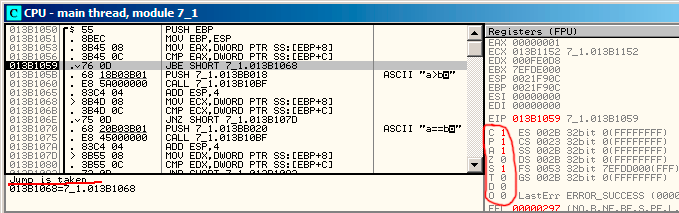
\includegraphics[scale=\FigScale]{patterns/07_jcc/simple/olly_unsigned1.png}
\caption{\olly: \TT{f\_unsigned()}: first conditional jump}
\label{fig:jcc_olly_unsigned_1}
\end{figure}

So, the flags are: C=1, P=1, A=1, Z=0, S=1, T=0, D=0, O=0.

They are named with one character for brevity in \olly.

\olly gives a hint that the (\JBE) jump is to be triggered now.
Indeed, if we take a look into Intel manuals (\myref{x86_manuals}), 
we can read there that \JBE is triggering if CF=1 or ZF=1.
The condition is true here, so the jump is triggered.

\clearpage
The next conditional jump:

\begin{figure}[H]
\centering
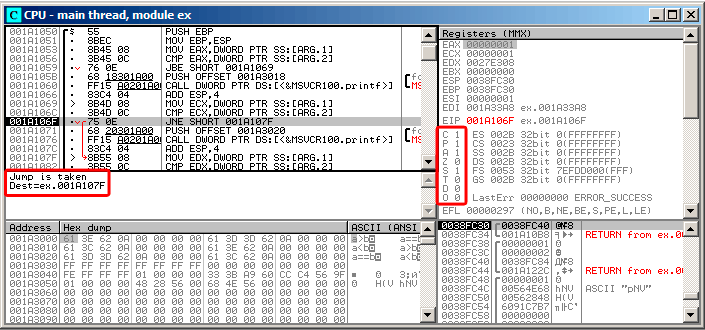
\includegraphics[scale=\FigScale]{patterns/07_jcc/simple/olly_unsigned2.png}
\caption{\olly: \TT{f\_unsigned()}: second conditional jump}
\label{fig:jcc_olly_unsigned_2}
\end{figure}

\olly gives a hint that \JNZ is to be triggered now.
Indeed, \JNZ triggering if ZF=0 (zero flag).

\clearpage
The third conditional jump, \JNB:

\begin{figure}[H]
\centering
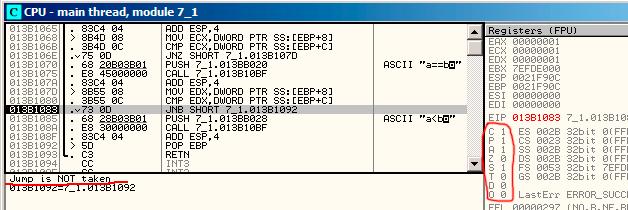
\includegraphics[scale=\FigScale]{patterns/07_jcc/simple/olly_unsigned3.png}
\caption{\olly: \TT{f\_unsigned()}: third conditional jump}
\label{fig:jcc_olly_unsigned_3}
\end{figure}

In Intel manuals (\myref{x86_manuals}) we can see that \JNB triggers if CF=0 (carry flag).
That is not true in our case, so the third \printf will execute.

\clearpage
Now let's review the \TT{f\_signed()} function, which works with signed values, in \olly.
Flags are set in the same way: C=1, P=1, A=1, Z=0, S=1, T=0, D=0, O=0.
The first conditional jump \JLE is to be triggered:

\begin{figure}[H]
\centering
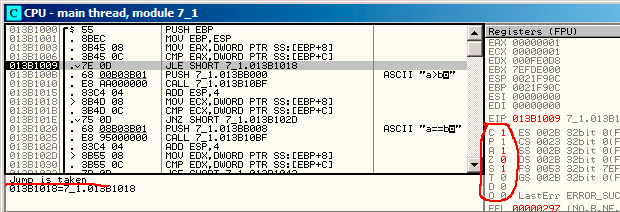
\includegraphics[scale=\FigScale]{patterns/07_jcc/simple/olly_signed1.png}
\caption{\olly: \TT{f\_signed()}: first conditional jump}
\label{fig:jcc_olly_signed_1}
\end{figure}

In Intel manuals (\myref{x86_manuals}) we find that this instruction is triggered if ZF=1 or SF$\neq$OF.
SF$\neq$OF in our case, so the jump triggers.

\clearpage
The second \JNZ conditional jump triggering: if ZF=0 (zero flag):

\begin{figure}[H]
\centering
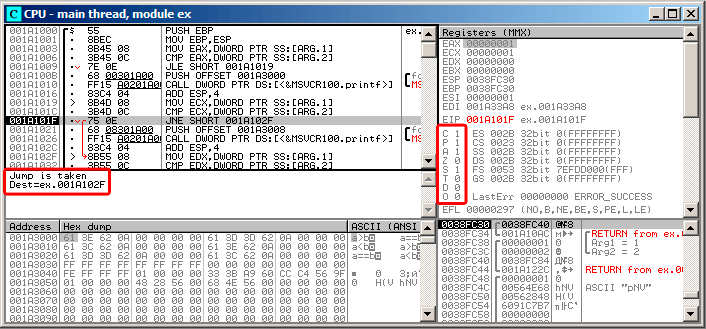
\includegraphics[scale=\FigScale]{patterns/07_jcc/simple/olly_signed2.png}
\caption{\olly: \TT{f\_signed()}: second conditional jump}
\label{fig:jcc_olly_signed_2}
\end{figure}

\clearpage
The third conditional jump \JGE will not trigger because it would only do so if SF=OF, and that is not true in our case:

\begin{figure}[H]
\centering
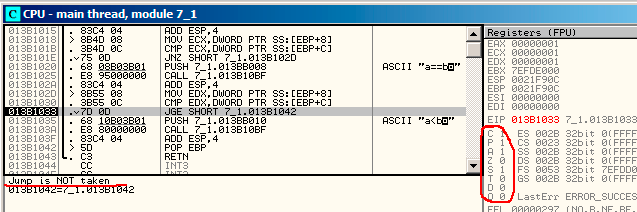
\includegraphics[scale=\FigScale]{patterns/07_jcc/simple/olly_signed3.png}
\caption{\olly: \TT{f\_signed()}: third conditional jump}
\label{fig:jcc_olly_signed_3}
\end{figure}
